\documentclass[a4paper]{article}

%\usepackage[english]{babel}
\usepackage[utf8]{inputenc}
\usepackage{amsmath}
\usepackage{graphicx}
\usepackage[colorinlistoftodos]{todonotes}
\usepackage[T1]{fontenc}	%ADDED for << og >>
\usepackage{enumitem}		%ADDED for smaller spacing
\usepackage[german]{babel}


\title{Assinment37}
\author{pebj, smot}
\date{\today}

\begin{document}
\maketitle


\begin{enumerate}
	\item Identify all relevant \textbf{Actors}.\\
    \begin{enumerate}[noitemsep,nolistsep]
        \item[1)]Client
        \item[2)]Server
        \item[3)]Moderater
    \end{enumerate}
	\item Identify and describe \textbf{2 non-trivial Scenarios}.\\
\end{enumerate}
    


\begin{tabular}{l r @{} l}
	\multicolumn{2}{c}{} \\
	\hline
	Scenario name	&&Entry sharing\\
	\hline
	Praticipating actor	&&Claus, Jan: Client \\
	instances       	&&\\
	\hline
	Flow of events	&1)&Claus' birthday is coming up, so he needs to invite any participants\\ 
					&&who would like to come. therefore he makes an event in the CALENDAR.\\
				&2)&When Claus have opened his CALENDAR, he uses the ''New event'' function.\\
                	&&which opens a new window for specifying the new event. \\
				&3)&He enters the date, place and a short discription of the event.\\
					&&Claus also choses a color for the event. A time he like to be alermed\\
					&&of the event and then he confirms his input.\\
				&4)&The CALENDAR closes the spicification window and shows Claus\\
					&& CALENDAR with his new event. Claus then uses the ''Share''\\
					&&function and gets a digital code he copyes and pasts it on hes\\
					&&Facebook wall.\\
				&5)&The friend Jan notices this digital code and wishes to take part in Claus' \\ 
					&&birthday. He therefore uses the digital code to get to a window, where he can\\
					&&chose to accept, which will put the event in his CALENDAR.\\
				&6)&Jan and Claus can now see the event in their calendar, with date, place,\\
					&&description and how many participants that have accepted the event.\\
	\hline
\end{tabular}
\\


\begin{tabular}{l r @{} l}
	\multicolumn{2}{c}{} \\
	\hline
	Scenario name	&&Upcomming event notification\\
	\hline
	Praticipating actor	&&Claus: Client \\
	instances       	&&server: Server\\
	\hline
	Flow of events	&1)&A week ago Claus inserted an event to his CALENDAR where he added\\ 
					&&an ''event alert'' to notify him 2 hours before the event.\\
				&2)&The server reacts to the ''event alert'' at the spicified time, by sending\\
					&&a message to the client Claus with the details for the upcomming event.\\
				&3)&Claus now gets a message notification in the form of an email etc.\\ 
				&4)&The message tells him of the upcomming event and shows him his CALENDAR\\
					&&for today.\\
	\hline
\end{tabular}

	\begin{enumerate}
		\item[3.] Identify all  relevant \textbf{Use Cases} and draw the \verb= "sticky man" UML= diagram.\\
		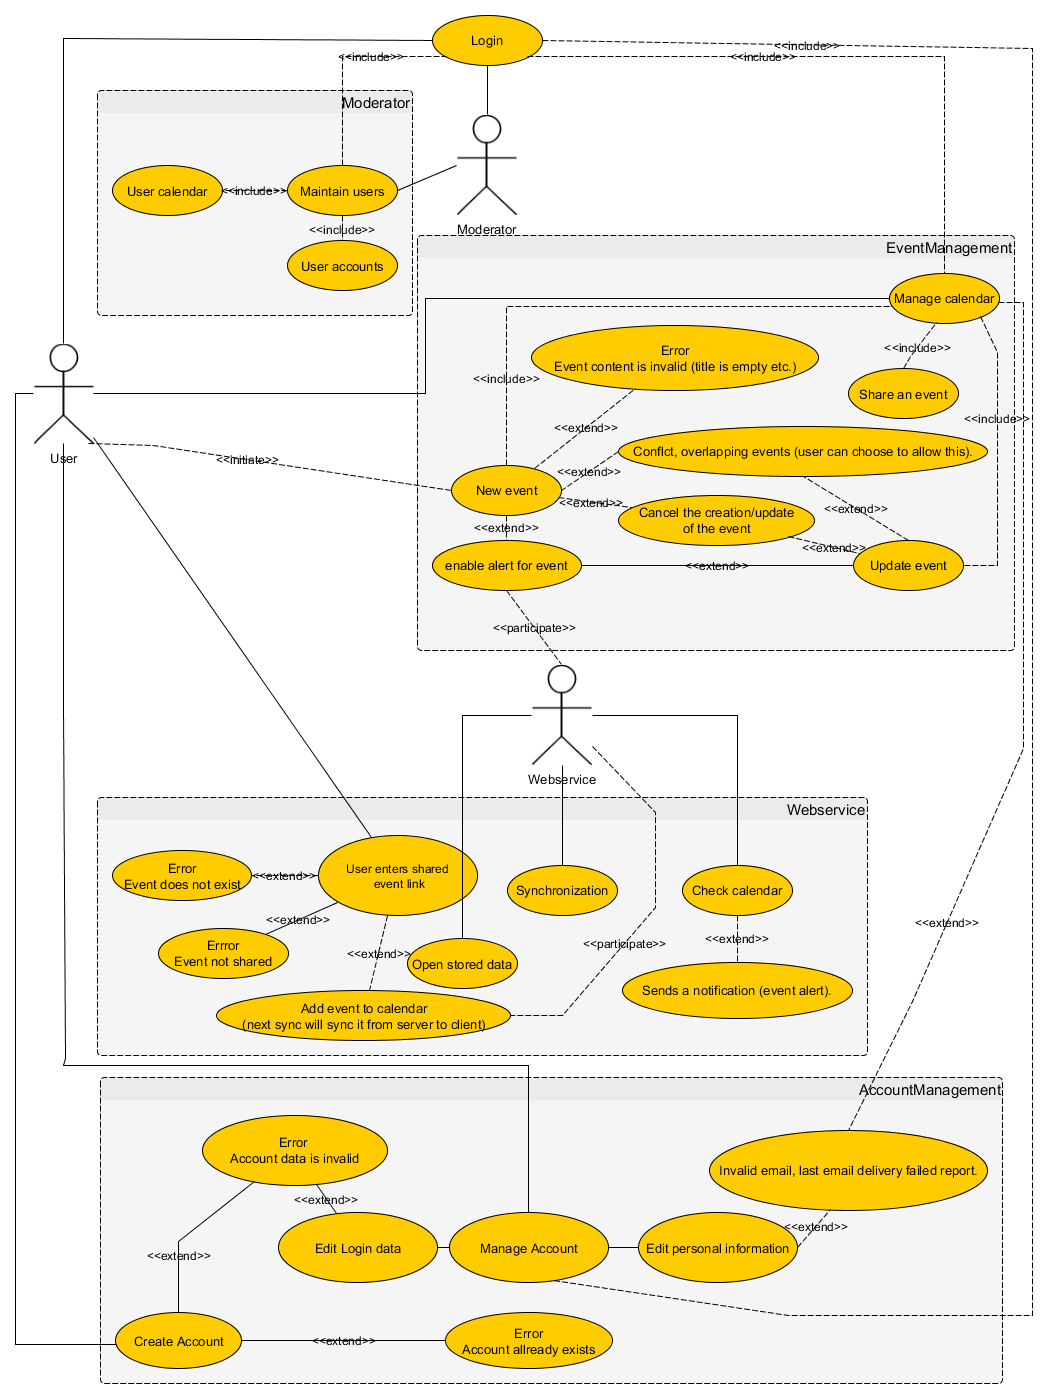
\includegraphics[scale = 0.38]{UserCases.png}\\
		\pagebreak{}
		\item[4.] Select 3 \textbf{non-trivial Use Cases} and document them using the use case table\\
	\end{enumerate}
\begin{tabular}{l r @{} l}
	\multicolumn{2}{c}{} \\
	4.1&&\\
	\hline
	Use case name:	&&Edit personal information (login data)\\
	\hline
	Participating actors:&&User \\
	\hline
	Flow of events:	&1.&User chooses to manage his account.\\
				&2.&User chooses to edit his/hers personal information.\\
	\hline
	Entry condition:	&&User is logged into the system.\\
	\hline
	Exit condition:	&&The user updates his personal information.\\
    &&Account data is invalid\\
	\hline
\end{tabular}
	\\
	.\\
\begin{tabular}{l r @{} l}
	\multicolumn{2}{c}{} \\
	4.2&&\\
	\hline
	Use case name:	&&Enable alert\\
	\hline
	Participating actors:&&User, Server \\
	\hline
	Flow of events:	&1.&User chooses to manage his calendar (login \flqq include\frqq has been profiled\\
				&&by entry condition). User chooses to add a new event.\\
				&2.&User chooses to enable an alert for his event (explained by the \flqq extend\frqq\\
					&& which tells us its an extension of the base case. You have to do the base case,\\
					&& but you may do the extension).\\
				&3.&The user chooses to enable the notification alert (due to the server participating\\
					&& in this, the server will act as an observer to your choice of enabling the event).\\
				&4.&You enable the alert and the server will know the result.\\
	\hline
	Entry condition:	&&User is logged into the system.\\
	\hline
	Exit condition:	&&The user chooses to enable/disable the alert.\\
    &&User cancels the creation/update of the event\\
	\hline
\end{tabular}
	\\
	.\\
\begin{tabular}{l r @{} l}
	\multicolumn{2}{c}{} \\
	4.3&&\\
	\hline
	Use case name:	&&Send event alert\\
	\hline
	Participating actors:&&Server\\
	\hline
	Flow of events:	&1.&Server checks the events for all users.\\
				&2.&On the condition that it finds an upcoming event, we will end up sending\\
					&&a notification to the user about it (using \flqq extend\frqq, we say\\
					&&that we arrive there as a condition is met,\\
					&&in this case, an event is an upcoming event).\\
	\hline
	Entry condition:	&&A timed loop chooses to have the server perform this task regularly.\\
	\hline
	Exit condition:	&&Event alerts have been sent for all upcoming events.\\
	\hline
\end{tabular}

	\pagebreak{}

\begin{enumerate}
		\item[5.] Identify \textbf{Relationships} between Actors and Use Cases and finalize the \verb= "sticky man"=  diagram\\
		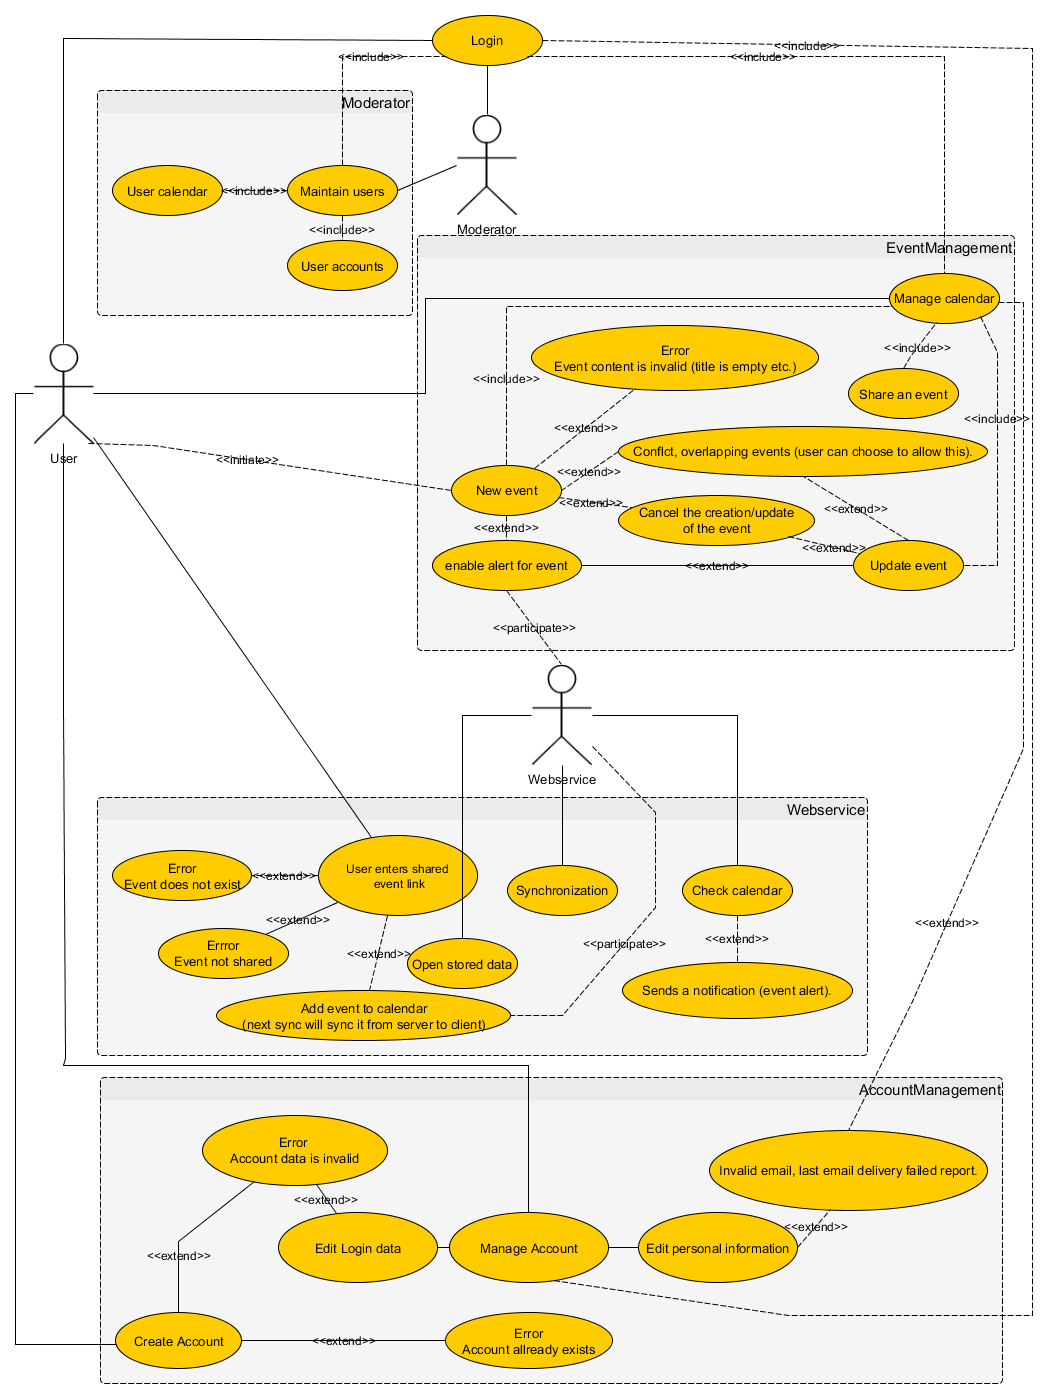
\includegraphics[scale = 0.38]{UserCases.png}\\
		\pagebreak{}
		\item[6.] Identify \textbf{Initial Analysis Objects} and document them in a table\\
\end{enumerate}

\begin{tabular}{l}
	\textbf{Participating objects for use cases 4.1, 4.2 and 4.3.}\\
	\hline
	\textbf{Server:} 
    Server activity which regularly checks up on all events and \\
	notifies users in case of an upcoming event. It is up to the user if he wants to have a notification sent,\\ 
	so the server will participate in the user’ events and choice of enabling the notification alert.\\ The server will also process shared events when a user enters a shared event link and\\
    add them to the user' calendar (read ''Shared event link'' for a more concrete explanation)\\
	\hline
	\textbf{User:} 
    the user can create events in his calendar. As such he is the initiator of event creation and \\
	other users may participate in those events if they are shared. \\
	Additionally a new possible event alert may be initiated which the server will participate in.\\
	\hline
    \textbf{Calendar:} 
    this system is where a user can store information on \textit{things} that is going to happen that\\
    he would like to keep track of. The \textit{things} is associated with a date and time that will\\
    happen,\textit{things} saved in this system are an event \\
	\hline
    \textbf{Event:} 
    a data entry that holds title, discription, dates for start, end and associated notifications to it.\\ It may also contain events as children as part of a composite pattern. \\
	\hline
    \textbf{Notification:} 
    Notifications can be an email etc. that is sent to the user when the current date\\
    exceeds the date property inside Notification.\\
    A notification is always associated with one particular event.\\
	\hline
    \textbf{Login:} 
    An action a user have to do to identify himself and show that he have authority to manipulate\\
    events associated with the account the user has logged in to. To login the user needs a username\\
    and a password, both associated with the account he like to login to. A moderator also need to\\
    login to show show that he have authority as a moderator.\\
	\hline
    \textbf{Account:} 
    Represents a user and contains events and notifications the user have. it also contains\\
    infomation about the user, however the password property of the account\\ must never be available to the client data structure.\\
	\hline
    \textbf{Shared event link:} 
    If the user wishes to share an event with friends and such, he can though\\
    his calendarsoftware generate a ''shared event link''. If anyone enters this link in a browser etc.\\
    a serverpage should appear asking for nessesary information for adding the event to the one who\\
    opened the link' calendar. Once done, a sync between client/server will get the shared event to\\
    appear in the user' calendar. A shared event can only be modified by its creator. Everyone else\\
    who is shared with are observers who can only remove it from their own calendar. \\
	\hline
\end{tabular}
	\\
\pagebreak


\begin{enumerate}
		\item[7.] Identify \textbf{Non-functional Requirements} and document them i a table\\
\end{enumerate}

\begin{tabular}{l r @{} l}
	\textbf{Non-functional Requirements}\\
	\hline
	\textbf{Usability:} Users must be able to view (not edit) a shared event without having an account\\
	 thus without logging in. The user interface should be kept simple, so fancy features should be kept\\
	 at a minimum. The only exception to the latter is if more features are kept isolated\\ 
	 from the simple interface, meaning that there may be a page dedicated for advanced features.\\
	\hline
	\textbf{Reliability:} The system may not make changes to the database in a way where a failure could\\
	 corrupt the database structure itself. For instance, if two changes were needed to complete a task and\\
	 only completing the first would cause the database to be corrupt, the software must not fail in\\
	 between those changes.\\
	\hline
	\textbf{Performance:} The asymptotic running time of the program must not increase propositionally\\
	by the number of events.\\
	\hline
	\textbf{Supportability:} The system must be designed in a way, so that new notifications types besides\\
	upcoming events notification can be implemented without the need to alter the implementation\\
	of the upcoming event notification.\\
	\hline
	\textbf{Implementation:} The implementation must work on\\
	at least one of the following main platform: Windows or Mac OS.\\
	\hline
	\textbf{Operation:} moderator maintains the users, but should be kept from seeing as much personal\\
	 information from users as possible unless specifically requested by the moderator.\\
	\hline
	\textbf{Legal:}  As in accordance to the Danish law \S 264,\\
	 it is not legal to forward messages or pictures concerning another person’ private circumstances\\
	 or pictures without permission from the person in question.\\ 
	This also means that the calendar system must not publicize/distribute the user’ events\\
	 or personal information (ads for software etc.) without the user’ personal permission.\\
	\hline
\end{tabular}

\end{document}